% Section 3 - Basic Communication
% Roberto Masocco <roberto.masocco@uniroma2.it>
% March 13, 2022

% ### Basic Communication ###
\section{Basic Communication}
\graphicspath{{figs/section3/}}

% --- ROS 2 Messages ---
\begin{frame}{ROS 2 Messages}
    \begin{block}{Definition of Message}
      A message is a \textbf{single DDS data packet} sent over a \textbf{topic}, from \textbf{publisher nodes} to \textbf{subscriber nodes}, with a specific \textbf{QoS policy}.
    \end{block}
    \begin{figure}
      \centering
      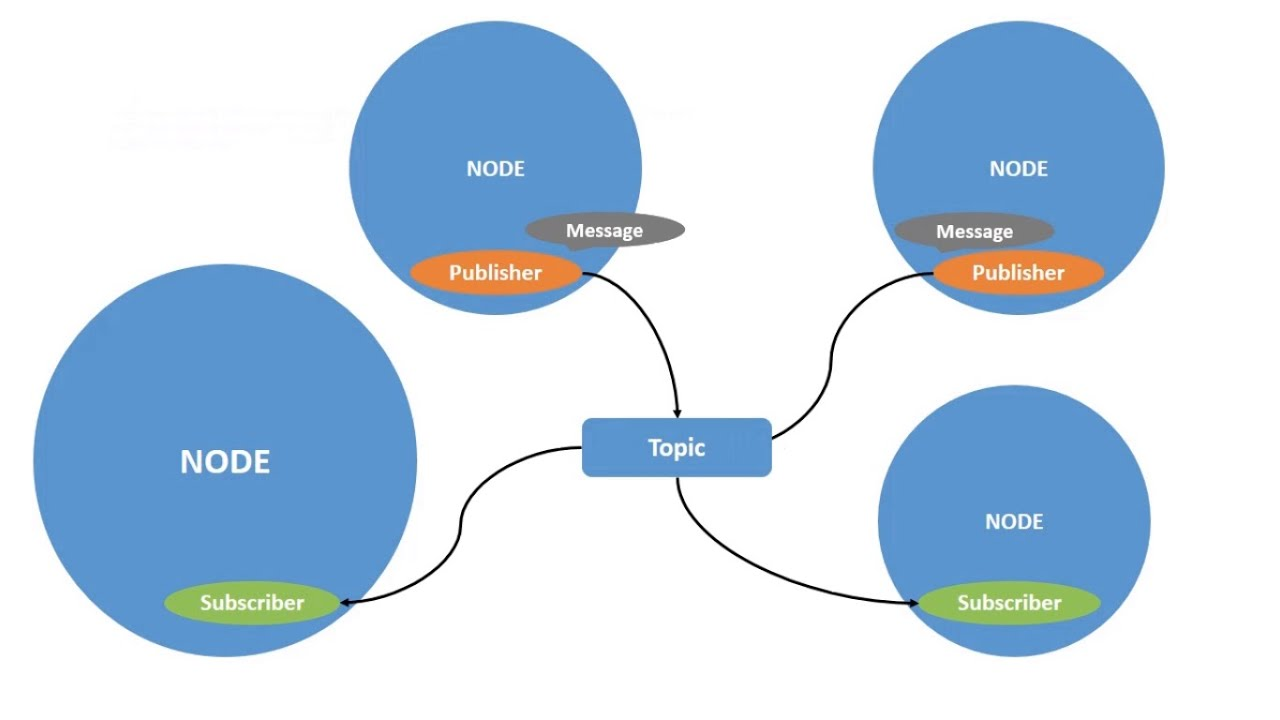
\includegraphics[scale=.19]{ros2Msg.jpg}
      \label{fig:msg}
      \caption{Example of a topic with multiple publisher and subscriber nodes}
    \end{figure}
\end{frame}

% --- Interface Files - Messages ---
\begin{frame}[fragile]{Interface Files - Messages}
Interface files format is specified by the DDS, with data types resolved to machine types according to the platform being used\footnote{\href{https://docs.ros.org/en/galactic/Concepts/About-ROS-Interfaces.html}{\color{blue}\underline{About ROS Interfaces}} (ROS 2 Galactic docs)}.\\
Things start very simply...

\begin{columns}
\column{.95\textwidth}
% Listing: std_msgs/msg/Int64 message definition
\begin{lstlisting}[language=ros2msg, caption=Definition of the \texttt{std\_msgs/msg/Int64} message]
int64 data
\end{lstlisting}

% Listing: std_msgs/msg/String message definition
\begin{lstlisting}[language=ros2msg, caption=Definition of the \texttt{std\_msgs/msg/String} message]
string data
\end{lstlisting}
\end{columns}

\end{frame}
\begin{frame}[fragile]{Interface Files - Messages}
... then escalate quickly!

\begin{columns}
\column{.95\textwidth}
% Listing: sensor_msgs/msg/Image
\begin{lstlisting}[language=ros2msg, caption=Definition of the \texttt{sensor\_msgs/msg/Image} composite message]
std_msgs/Header header

uint32 height
uint32 width

string encoding

uint8 is_bigendian
uint32 step
uint8[] data
\end{lstlisting}
\end{columns}

\end{frame}
\begin{frame}[fragile]{Interface Files - Messages}
Special values (i.e. constants) may be specified.

\begin{columns}
\column{.95\textwidth}
% Listing: message with constant
\begin{lstlisting}[language=ros2msg, caption=Definition of an example message with a constant value]
int64 MYNUM=1 # Must be of compatible type

int64 number
\end{lstlisting}
\end{columns}

They are not bound to any field and will appear as special selectable values in the generated C++/Python libraries.\\
ROS 2 adds its own guidelines\footnote{\href{https://github.com/IntelligentSystemsLabUTV/ros2-examples/blob/galactic/interfaces.md}{\color{blue}\underline{ros2-examples/interfaces.md}}}, and installed interfaces can be inspected with the \texttt{ros2 interface show} command.
\end{frame}
